%%%%%%%%%%%%%%%%%%%%%%%%%%%%%%%%%%%%%%%%%%%%%%%%%%%%%%%%%%%%%%%%%%%%%%%%%%%%%%%%
\section{Why Workflows}

%%%%%%%%%%%%%%%%%%%%%%%%%%%%%%%%%%%%%%%%%%%%%%%%%%%%%%%%%%%%%%%%%%%%%%%%%%%%%%%%
\begin{frame}
    \frametitle{Outline}
    \begin{columns}[t]
        \begin{column}{.5\textwidth}
            \tableofcontents[sections={1-7},currentsection]
        \end{column}
        \begin{column}{.5\textwidth}
            \tableofcontents[sections={8-15},currentsection]
        \end{column}
    \end{columns}
\end{frame}

%%%%%%%%%%%%%%%%%%%%%%%%%%%%%%%%%%%%%%%%%%%%%%%%%%%%%%%%%%%%%%%%%%%%%%%%%%%%%%%%
\begin{frame}
  \frametitle{What is this about?}
   \begin{question}[Questions]
   	 \begin{itemize}
        \item Let them learn the batch system! Really?
        \item What is the benefit of a workflow system for admins?
        \item What distinguishes a workflow system from a ``pipeline''?
     \end{itemize}
   \end{question}
   \begin{docs}[Objectives]
   	  \begin{enumerate}
         \item Introducing workflow engines (particularly \Snakemake)!
      \end{enumerate}
   \end{docs}
\end{frame}  

%%%%%%%%%%%%%%%%%%%%%%%%%%%%%%%%%%%%%%%%%%%%%%%%%%%%%%%%%%%%%%%%%%%%%%%%%%%%%%%%
\begin{frame}
  \frametitle{Data Analysis}
  \begin{onlyenv}<1| handout:0>
    \begin{tikzpicture}
      \path[use as bounding box] (0.7,0) rectangle (12,8);
      \node[inner sep=0pt] (analysis_1) at (5,6)
         {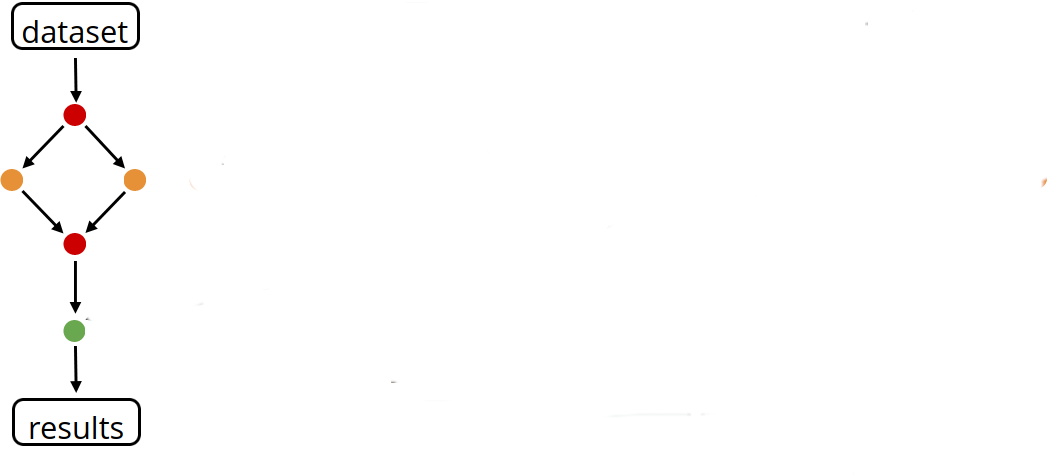
\includegraphics[width=0.7\textwidth]{Snakemake/analysis_1.png}};   
      \node at (7, 3.5) %[below=-0.4cm of analysis_1, xshift=2.7cm] at (current page.center)
         {
\includegraphics[width=0.45\textwidth]{Snakemake/phd_left.png}};
      \node at (6, 1) {\begin{minipage}{0.75\textwidth}\footnotesize
                        Idea from the official \lhref{https://slides.com/johanneskoester/snakemake-tutorial}{\Snakemake} course (with permission), image from \lhref{https://phdcomics.com/comics.php}{PhD comics}.
                       \end{minipage}
      };
    \end{tikzpicture}    
  \end{onlyenv}
  
  \begin{onlyenv}<2| handout:1>
    \begin{tikzpicture}
      \path[use as bounding box] (0.7,0) rectangle (12,8);
      \node[inner sep=0pt] (analysis_full) at (5,6)
         {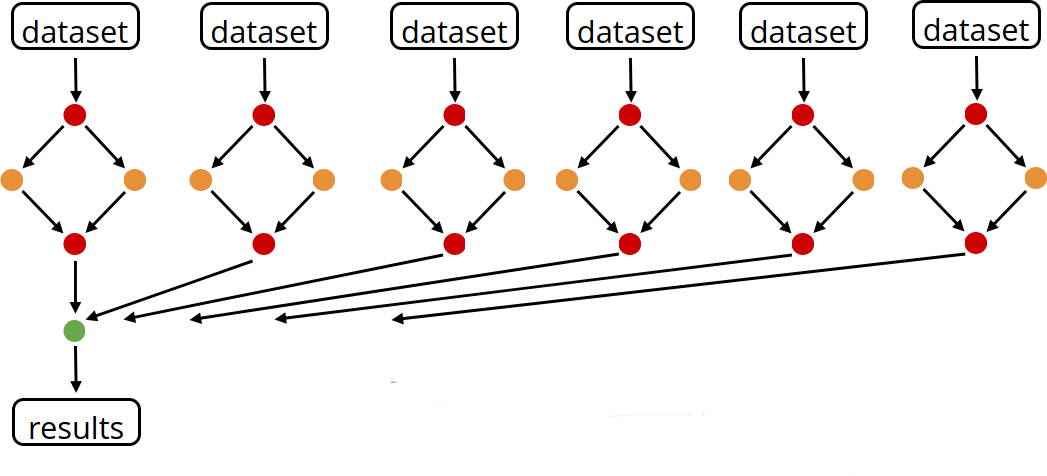
\includegraphics[width=0.7\textwidth]{Snakemake/analysis_full.png}};   
      \node at (7,3.5) % [below=-0.4cm of analysis_full, xshift=2.7cm]
         {
\includegraphics[width=0.45\textwidth]{Snakemake/phd_full.png}};
      \node at (6, 1) {\begin{minipage}{0.75\textwidth}\footnotesize
                        Idea from the official \lhref{https://slides.com/johanneskoester/snakemake-tutorial}{\Snakemake} course (with permission), image from \lhref{https://phdcomics.com/comics.php}{PhD comics}.
                       \end{minipage}
      };
    \end{tikzpicture}
  \end{onlyenv}
\end{frame}

%TODO Here, I (CM) wanted to introcue a slide with a DAG 

%%%%%%%%%%%%%%%%%%%%%%%%%%%%%%%%%%%%%%%%%%%%%%%%%%%%%%%%%%%%%%%%%%%%%%%%%%%%%%%%
\begin{frame}
	\frametitle{Data Analysis - Using a Batch System???}
	\begin{columns}
		\begin{column}{0.5\textwidth}
			\begin{tikzpicture}
				\path[use as bounding box] (0.7,0) rectangle (12,8);
				\node[inner sep=0pt] (analysis_full) at (4,6)
				{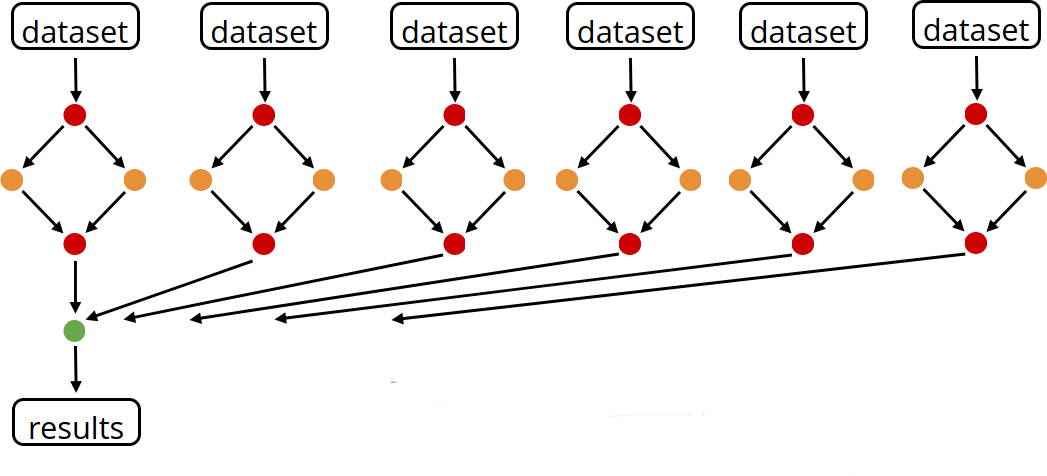
\includegraphics[width=0.7\textwidth]{Snakemake/analysis_full.png}}; 
			\end{tikzpicture}
		\end{column}
	    \begin{column}{0.5\textwidth}
	    A workflow with 1 shepherd (master), 11 jobs scripts (for multiple, concurrent execution, incl. dependency handling) was coded by one student:
	    \begin{itemize}[<+->]
	    	\item ca. 4400 lines of Bash
	    	\item 1 Perl script: 240 lines
	    	\item 1 Python script: 57 lines
	    \end{itemize}
      
	    \end{column}	
	\end{columns}
	\vspace{-12.5em}
	\begin{columns}
		\begin{column}{0.5\textwidth}
			  \pause
			\begin{question}
				How portable is this? How maintainable? How many people are able to accomplish this?\\\pause\hline\vspace{0.5em}
				
				Which conclusions will your users in need of complex analysis steps draw?
			\end{question}	
		\end{column}
		\begin{column}{0.5\textwidth}
			%empty
		\end{column}
	\end{columns}
\end{frame}	

%%%%%%%%%%%%%%%%%%%%%%%%%%%%%%%%%%%%%%%%%%%%%%%%%%%%%%%%%%%%%%%%%%%%%%%%%%%%%%%%
\begin{frame}
  \frametitle{Let them learn! Really?}
  \bcinfo Contemplate \ldots
  \pause
  \begin{question}[When do new users apply for HPC time?]
  	\pause With BIG DATA - or HUGE SIMULATIONS - not for anything else!
  \end{question}
  \pause
  \begin{question}[What do users expect to analyze their data?]
  	\begin{itemize}[<+->]
  		\item all necessary software -- no install hiccups
  		\item to \emph{just} calculate -- no complaints about IO issues or the like
  		\item to get their results \emph{fast} -- after all, it's an HPC system!
  	\end{itemize}
  \end{question}
  \pause
  \begin{question}[What will users think, if their expectations aren't met?]
  	\begin{itemize}[<+->]
  		\item what a workload compared to "my server"??
  		\item what a workload to get here (bureaucracy) and now this??
  		\item abandon HPC!
  	\end{itemize}
  \end{question}	
\end{frame}	

%%%%%%%%%%%%%%%%%%%%%%%%%%%%%%%%%%%%%%%%%%%%%%%%%%%%%%%%%%%%%%%%%%%%%%%%%%%%%%%%
\begin{frame}
  \frametitle{Let them learn! Really? - II}
  \begin{question}[How do users plan?]
	\begin{itemize}[<+->]
		\item is data management accounted for?
		\item are their jobs always (well enough) parameterized?
		\item where do get they their infos from? The "internet"? A labmate? A PI?
	\end{itemize}	
  \end{question}
  \pause
  \begin{question}[How do you meet expectations?]
    \begin{itemize}[<+->]
      \item software provisioning schemes
      \item data management support
      \item curated workflows
      \item every item feasible to which extend? With your manpower?
    \end{itemize}
  \end{question}
\end{frame}	


%%%%%%%%%%%%%%%%%%%%%%%%%%%%%%%%%%%%%%%%%%%%%%%%%%%%%%%%%%%%%%%%%%%%%%%%%%%%%%%%
\begin{frame}
  \frametitle{Reproducible Data Analysis in an OpenScience World}
  \begin{onlyenv}<1| handout:0>
    \begin{tikzpicture}
      \path[use as bounding box] (0.7,0) rectangle (12,8);
      \node at (5.5, 5.5) {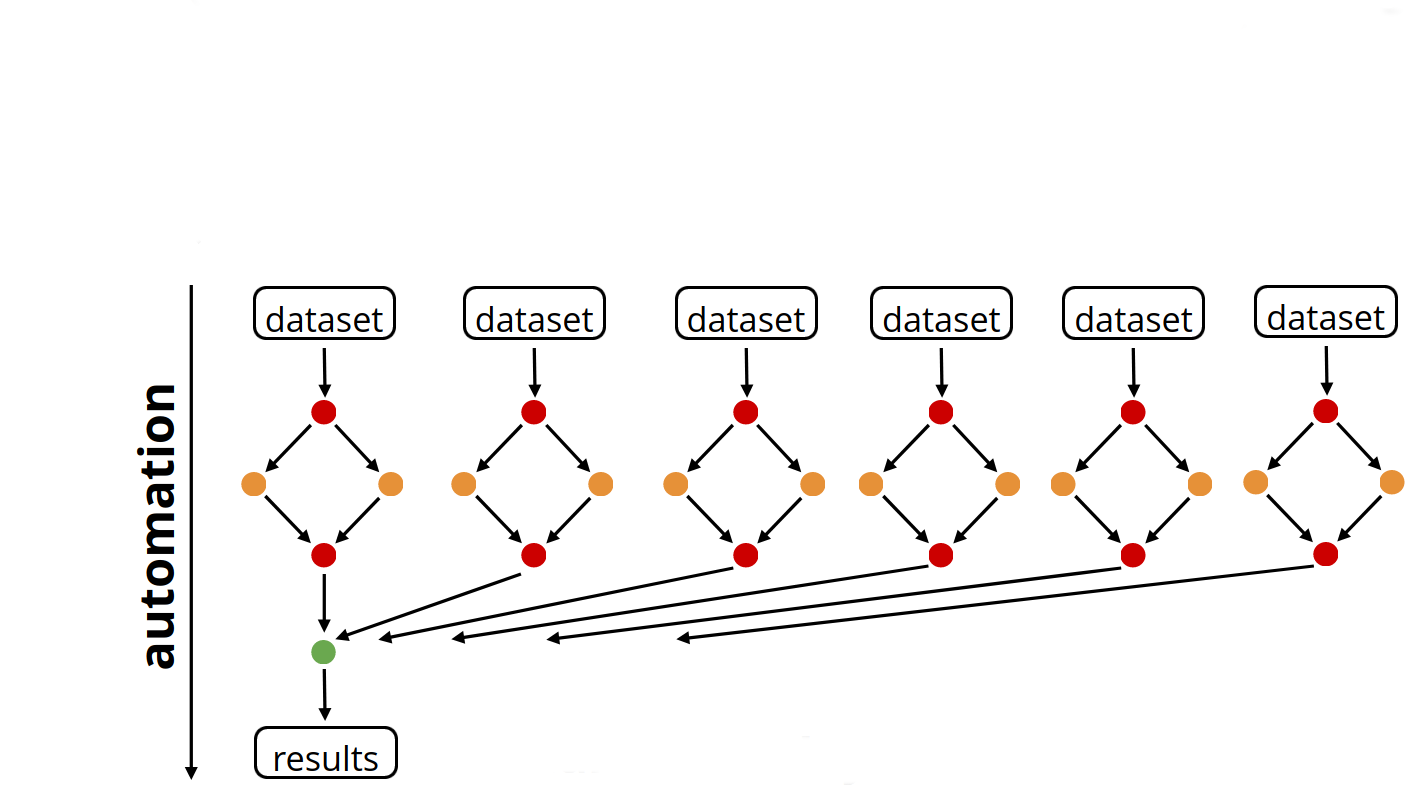
\includegraphics[width=0.7\textwidth]{Snakemake/automation.png}};
      \node at (8, 2.5) {\begin{minipage}{0.65\textwidth}
                             \textbf{From raw data to final figures:}
                             \begin{itemize}
                                \item \textbf{document} parameters, tools, versions
                                \item \textbf{execute} without manual intervention
                              \end{itemize}
                           \end{minipage}
                           };
    \end{tikzpicture}
  \end{onlyenv}
  \begin{onlyenv}<2| handout:0>
    \begin{tikzpicture}
      \path[use as bounding box] (0.7,0) rectangle (12,8);
      \node at (5.5, 5.5) {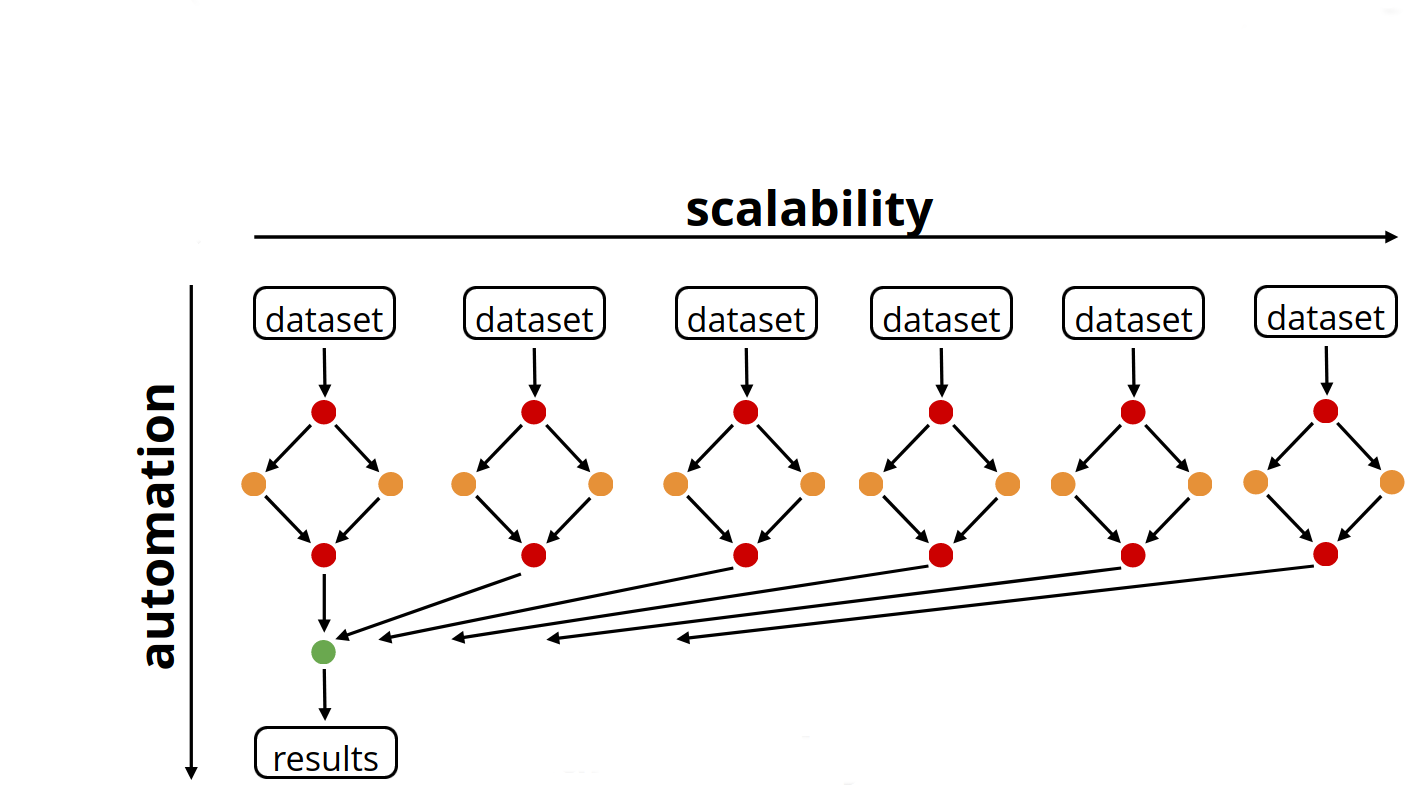
\includegraphics[width=0.7\textwidth]{Snakemake/scalability.png}};
      \node at (8, 2.5) {\begin{minipage}{0.65\textwidth}
                             \textbf{Handle parallelization:}
                             \begin{itemize}
                                \item execute for tens of thousands of datasets
                                \item efficiently use any computing platform
                              \end{itemize}
                           \end{minipage}
                           };
    \end{tikzpicture}
  \end{onlyenv}
  \begin{onlyenv}<3| handout:1>
    \begin{tikzpicture}
      \path[use as bounding box] (0.7,0) rectangle (12,8);
      \node at (5.5, 5.5) {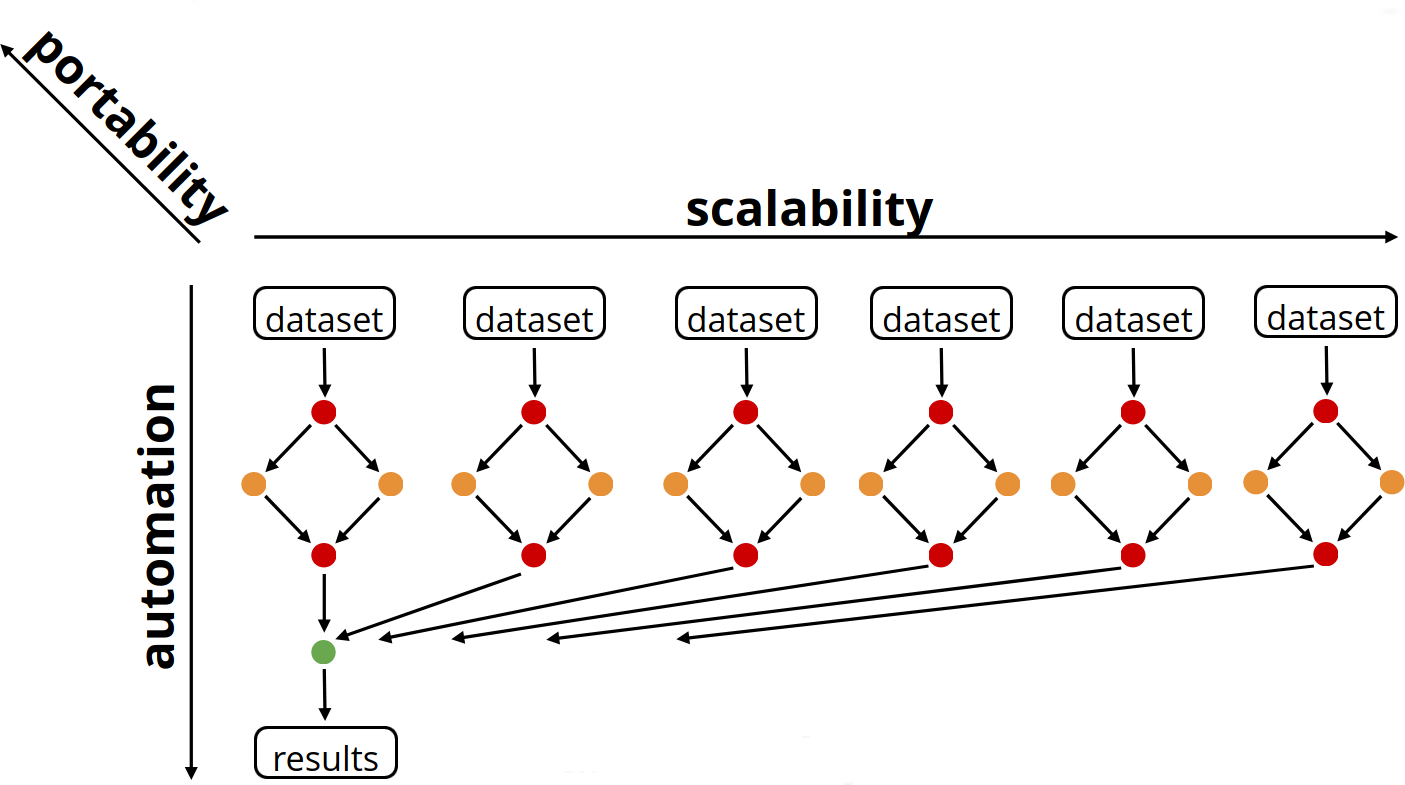
\includegraphics[width=0.7\textwidth]{Snakemake/portability.png}};
      \node at (8, 2.5) {\begin{minipage}{0.65\textwidth}
                             \textbf{Handle deployment:}\newline
                             be able to easily execute analyses on a different system/platform/infrastructure
                           \end{minipage}
                           };
    \end{tikzpicture}
  \end{onlyenv}
\end{frame}

%%%%%%%%%%%%%%%%%%%%%%%%%%%%%%%%%%%%%%%%%%%%%%%%%%%%%%%%%%%%%%%%%%%%%%%%%%%%%%%%
\begin{frame}
  \frametitle{Beyond Reproducibility}
  \begin{onlyenv}<1| handout:0>
    \begin{figure}
      \centering
      
\includegraphics[width=0.85\textwidth]{Snakemake/reproducibility_only.png}
    \end{figure}
  \end{onlyenv}
  \begin{onlyenv}<2| handout:0>
    \begin{figure}
      \centering
      
\includegraphics[width=0.85\textwidth]{Snakemake/reproducibility_empty.png}
    \end{figure}
  \end{onlyenv}
  \begin{onlyenv}<3| handout:0>
    \begin{figure}
      \centering
      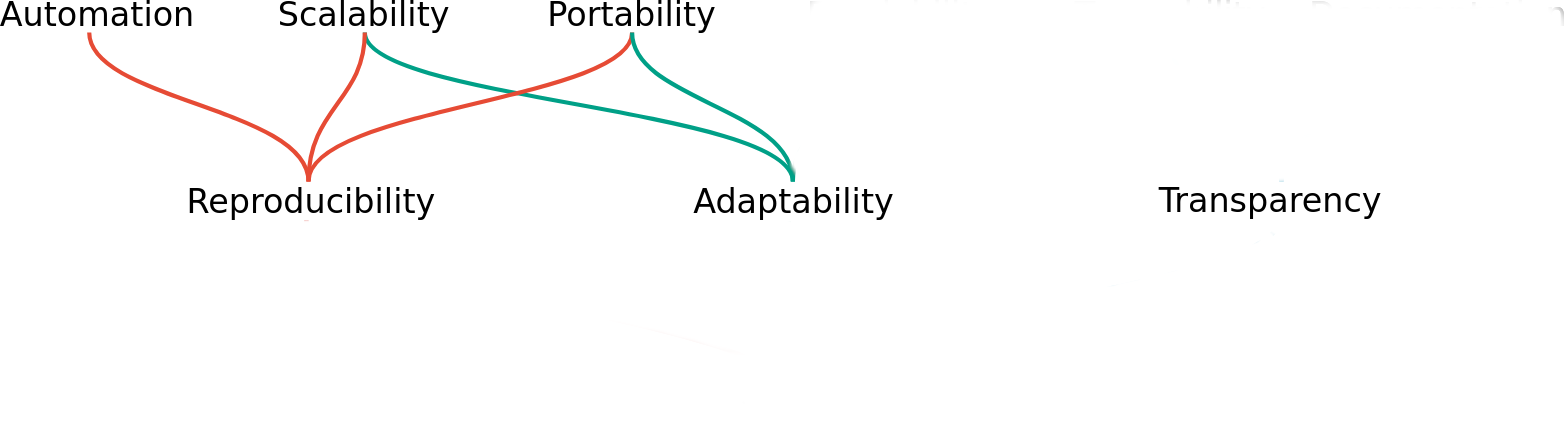
\includegraphics[width=0.85\textwidth]{Snakemake/reproducibility_left.png}
    \end{figure}
  \end{onlyenv}
    \begin{onlyenv}<4| handout:1>
      \begin{figure}
        \centering
        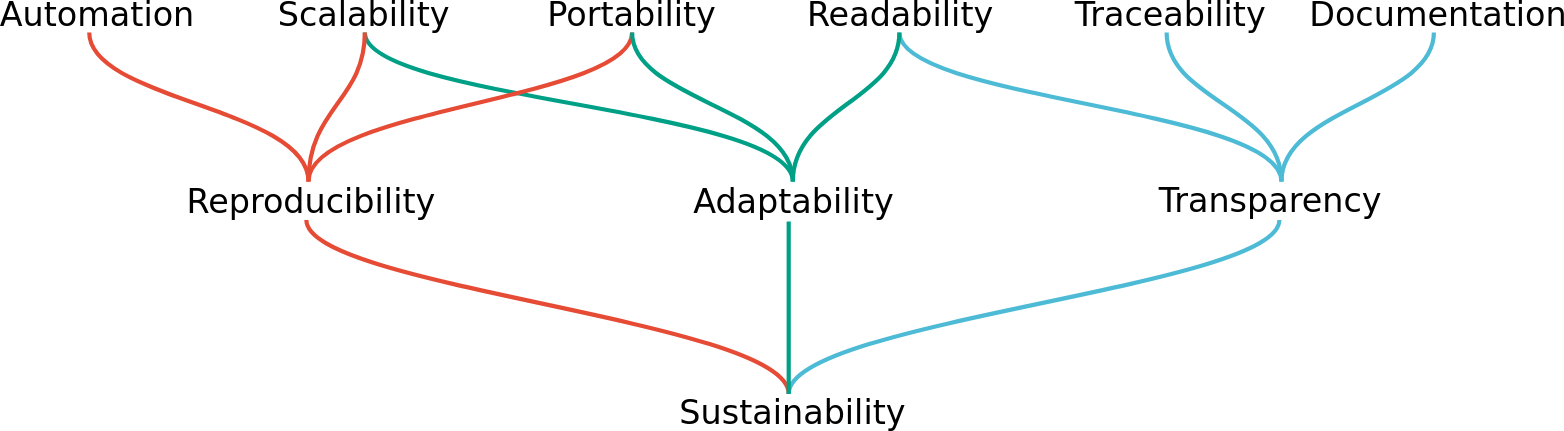
\includegraphics[width=0.85\textwidth]{Snakemake/reproducibility_full.png}
      \end{figure}
  \end{onlyenv}
  \footnotesize{\lhref{https://doi.org/10.12688/f1000research.29032.2}{From the official \Snakemake-paper.}}
\end{frame}
